\chapter{Vergleich der verschiedenen Implementierungen}
\label{chapter:4}

Wir haben im vorherigen Kapitel drei verschiedene Programmiersprachen bzw. Softwarebibliotheken vorgestellt und gezeigt, wie man dort Regressionsanalyse betreiben kann. In diesem Kapitel wollen wir zum Einen konkret auf die Unterschiede eingehen und zum anderen einen Benchmark bezüglich der Laufzeit abhängig von der Anzahl der zu verarbeitenden Datensätze erstellen.

\section{Iterative und explizite Berechnung}
\label{section:4:1}

Wir haben hier zwei verschiedene Arten zur Berechnung der Parameter verwendet. Bei expliziten Berechnungen wurden verschiedene Berechnungsformeln ausgewertet, bei iterativer Berechnung wurden Optimierungsverfahren verwendet, um die Werte gesuchten Parameter Schritt für Schritt besser zu approximieren.

In R haben wir ausschließlich explizite Berechnungen durchgeführt. Dazu haben wir die bereits implenentierten Funktionen $lm$ und $glm$ verwendet.

In TensorFlow kamen dagegen ausschließlich iterative Berechnungen zum Einsatz, TensorFlow ist ja auch eine Bibliothek, die für diesen Zweck programmiert wurde. Wir haben ein von TensorFlow implementiertes Gradientenverfahren genutzt, um eine jeweils von uns definierte Kostenfunktion zu minimieren oder zu maximieren. Die Kostenfunktionen waren dabei die Summe der kleinsten Quadrate bei linearer Regression und die Likelihoodfunktion bei logistischer Regression.

In SQL haben wir beide Berechnungsarten umgesetzt. Bei linearer Regression haben wir die expliziten Formeln aus den Kapiteln \ref{subsection:2:1:1} und \ref{subsection:2:1:2} verwendet. Bei logistischer Regression wurde wiederum ein Gradientenverfahren angewandt, nur dieses Mal wurde das Verfahren eigens implementiert, nachdem SQL nicht über ein solche Funktion verfügt.

\section{Benchmarking}
\label{section:4:2}

Nun wollen wir die konkreten Laufzeiten für die implememtierten Algorithmen vergleichen. Zu erwarten ist auf jeden Fall, dass Skripte unter Verwendung von iterativen Verfahren länger laufen als solche mit expliziter Berechnung. Außerdem ist zu vermuten, dass die eigenen Implementierungen in SQL langsamer sind, als wie die vorprogrammierten Funktionen in R und TensorFlow.

Zur Berechnung der Laufzeiten wurde erneut ein Python-Skript geschrieben. Dieses Skript führt die jeweilige Regression über einen Kommandozeilenbefehl aus und misst die Zeit dieser Operation. Die Anzahl der Wiederholungen und die Anzahl der verwendeten Datenpunkte können als Parameter übergeben werden. Die Ergebnisse der Berechnungen werden als csv-Datei gespeichert. Das Skript findet man im Anhang unter \ref{appendix:F:1}.

Auch für das Auswerten der berechneten Benchmarks wurde ein Python-Skript erstellt. Dieses Skript liest eine csv-Datei mit Benchmarks ein und druckt eine Tabelle mit den Werten für jede Art der Regression. Außerdem werden mehrere Plots für die Lautzeiten erzeugt. Alle Benchmarks wurden auf einem MacBook Pro (Mitte 2012) mit einem 2,9 GHz Intel Core i7 Prozessor und 8 GB 1600 MHz DDR3 Arbeitsspeicher berechnet.

\subsection{Einfache lineare Regression}
\label{subsection:4:2:1}

Folgende Benchmarks erhalten wir bei einfacher linearer Regression:

\begin{center}
  \captionof{table}{Benchmarks für einfache lineare Regression}
  \begin{tabular}{|c|c|c|c|c|c|}\hline
    & \textbf{10} & \textbf{100} & \textbf{1000} & \textbf{10000} & \textbf{100000} \\ \hline
    \textbf{r} & 0.38453477 & 0.40336191 & 0.38638819 & 0.40475887 & 0.54730985 \\ \hline
    \textbf{tensorflow} & 2.96190362 & 2.94665535 & 3.00290149 & 3.69807061 & 7.73616447 \\ \hline
    \textbf{mysql} & 0.02591379 & 0.02506811 & 0.03348756 & 0.11362195 & 0.82149320 \\ \hline
    \textbf{postgresql} & 0.03092405 & 0.03056195 & 0.03340294 & 0.04948901 & 0.21394655 \\ \hline
  \end{tabular}
\end{center}

Der zugehörige Graph (mit logarithmischen Skalen) sieht folgendermaßen aus:

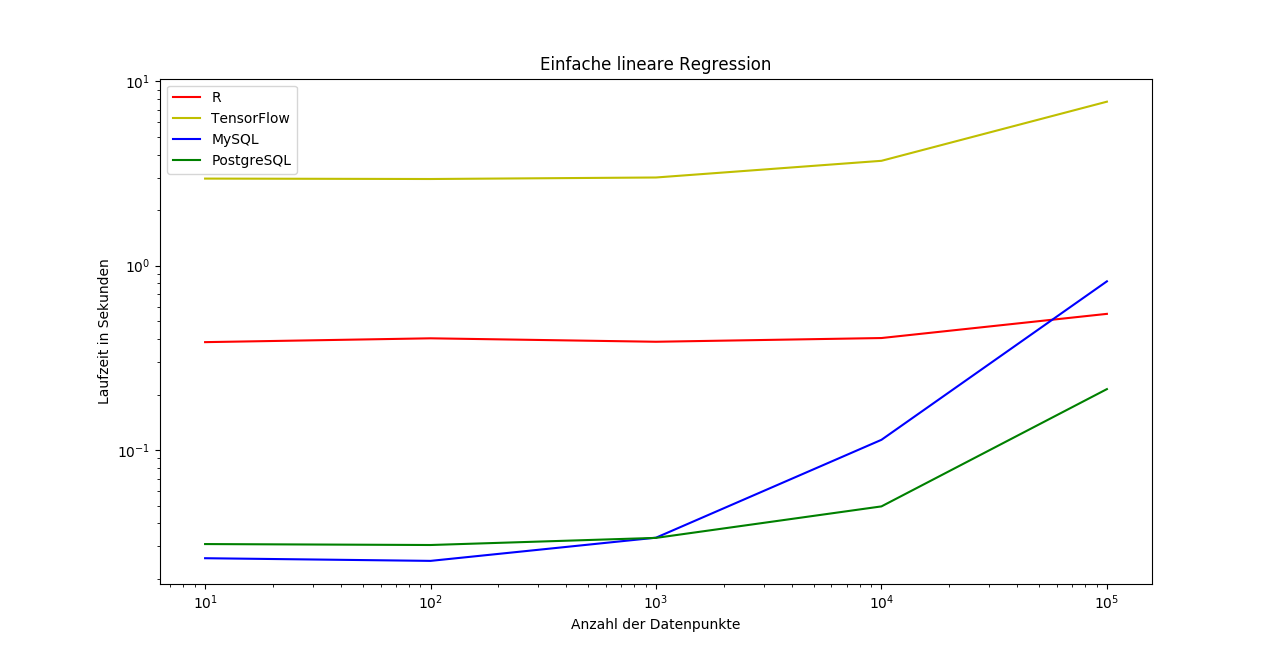
\includegraphics[width=\textwidth]{simpleLinearRegressionBenchmark}

TensorFlow und R haben eine relativ konstante Lautzeit, auch be größeren Datenmengen. Dabei ist TensorFlow mit iterativer Berechnung wie erwartet mit Abstand am langsamsten. Die SQL-Implementierungen sind bei geringer Anzahl an Datenpunkten sogar die schnellsten Skripte. Für größer werdende Datenmengen erkennt man aber einen rapiden Anstieg in der Lautzeit.

\subsection{Multiple lineare Regression}
\label{subsection:4:2:2}

Die Skripte für multiple lineare Regression besitzten folgende Laufzeiten:

\begin{center}
  \captionof{table}{Benchmarks für multiple lineare Regression}
  \begin{tabular}{|c|c|c|c|c|c|}\hline
    & \textbf{10} & \textbf{100} & \textbf{1000} & \textbf{10000} & \textbf{100000} \\ \hline
    \textbf{r} & 0.38108478 & 0.37967851 & 0.38452695 & 0.39888490 & 0.54517789 \\ \hline
    \textbf{tensorflow} & 167.676894 & 168.226441 & 167.186729 & 169.817689 & 167.200023 \\ \hline
    \textbf{mysql} & 0.04174929 & 0.05248516 & 0.15990342 & 1.09634777 & 10.8214030 \\ \hline
    \textbf{postgresql} & 0.03053954 & 0.03336087 & 0.05904620 & 0.30572490 & 2.71992954 \\ \hline
  \end{tabular}
\end{center}

Das geplottete Ergebnis sieht wiefolgt aus:

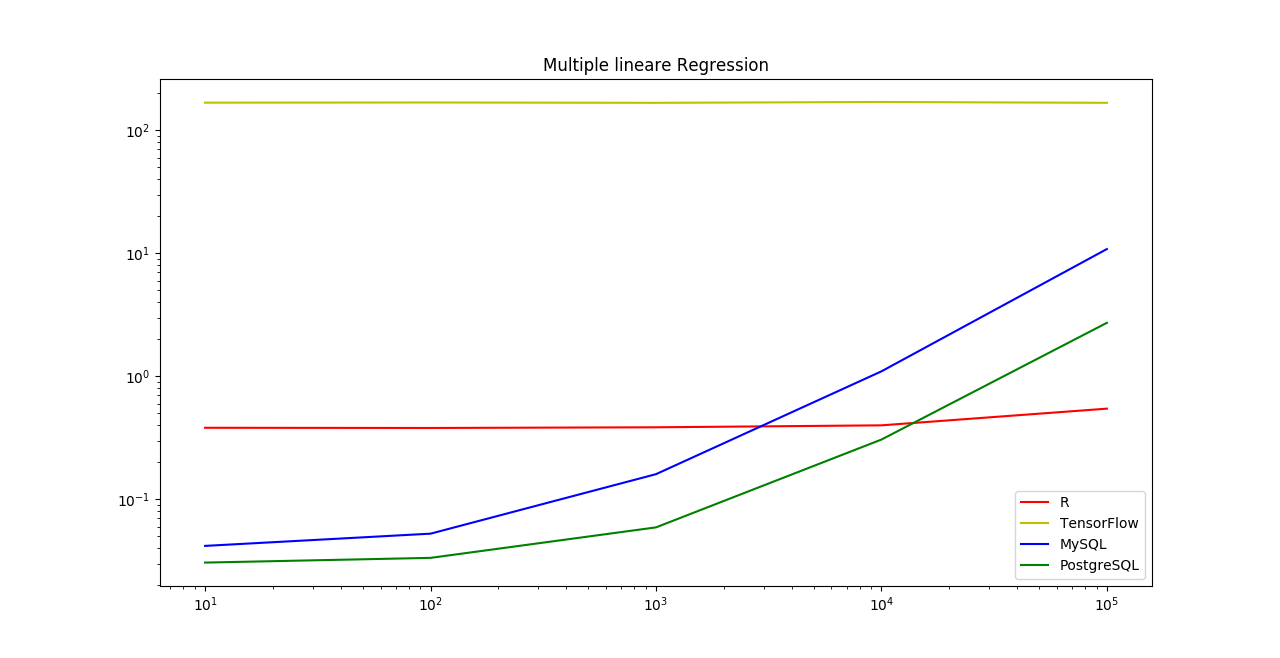
\includegraphics[width=\textwidth]{multipleLinearRegressionBenchmark}

Hier zeigt sich ein ähnliches Bild wie schon bei einfacher lineare Regression. Wieder liefern R und TensorFlow relativ konstante Laufzeiten, wobei die Laufzeit des TensorFlow-Skriptes wegen den $50.000$ durchgeführten Iterationen dieses Mal extrem langsam ist. Wieder sind die SQL-Skripte bei kleinen Datenmengen am schnellsten. Bei größeren Datenmengen werden sie allerdings von R geschlagen. Interessant ist außerdem, dass die PostgreSQL-Implementierung noch schneller als die Variante in MySQL. Die Arrays von PostgreSQL arbeiten also effizienter als die temporären Tabellen in MySQL.

\subsection{Logistische Regression}
\label{subsection:4:2:3}

Betrachten wir zuletzt noch einige Benchmarks für logistische Regression:

\begin{center}
  \captionof{table}{Benchmarks für logistische Regression}
  \begin{tabular}{|c|c|c|c|c|c|}\hline
    & \textbf{10} & \textbf{100} & \textbf{1000} & \textbf{10000} & \textbf{100000} \\ \hline
    \textbf{r} & 0.40403676 & 0.39953323 & 0.40047518 & 0.43356463 & 0.91014730 \\ \hline
    \textbf{tensorflow} & 2.88191271 & 2.88278436 & 2.92470042 & 3.37794654 & 6.87024382 \\ \hline
    \textbf{mysql} & 1.57908838 & 4.51631200 & 35.3472805 & 283.849979 & \\ \hline
    \textbf{postgresql} & 3.73521209 & 48.8452754 & 526.125703 & & \\ \hline
  \end{tabular}
\end{center}

Das visualisierte Pondon der Tabelle sieht so aus:

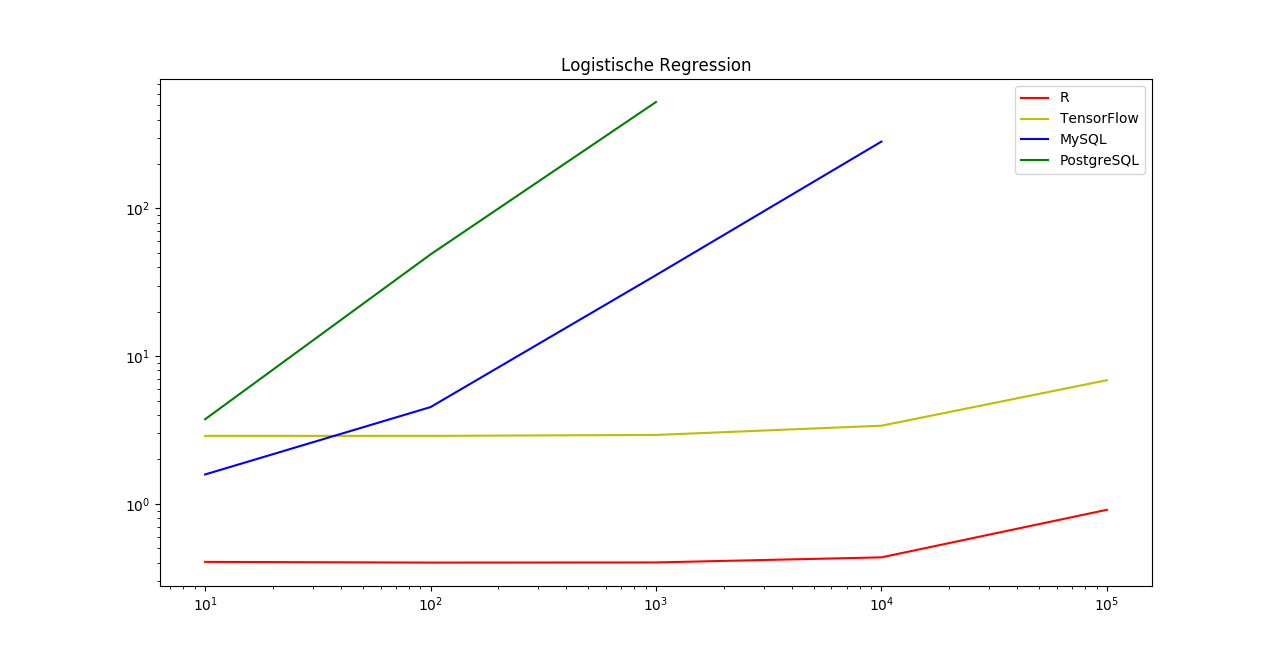
\includegraphics[width=\textwidth]{logisticRegressionBenchmark}

Wieder erkennt man eine Ähnlichkeit zu den vorherigen Diagrammen. Die SQL-Implementierungen sind nun aber von Anfang an deutlich langsamer als die Skripte in R und TensorFlow. Die Laufzeit steigt außerdem sehr schnell weiter an. So wurden für ab $10.000$ Datenpunkte gar keine Benchmarks mehr berechnet, da die erwartete Laufzeit länger als eine Stunde beträgt. Klarer Gewinner ist hier R, wo auch $100.000$ Datenpunkte in weniger als einer Sekunde verarbeitet werden können.
